\documentclass{beamer}
\usepackage[utf8]{inputenc}
\usepackage[portuguese]{babel}
\usepackage{amsmath}
\usepackage{subfigure}
\usepackage{booktabs}
\usepackage{mhchem}             % chemical reactions
\usetheme{metropolis}           % Use metropolis theme
\usepackage{animate}
\usepackage{xmpmulti}

\newtheorem{mydefinition}{Definição}

\newcommand{\foreignword}[1]{\textit{#1}}
\newcommand{\toolname}[1]{\textit{#1}}
\newcommand{\fieldR}{\mathbb{R}}
\newcommand{\powerset}{\mathcal{P}}
\newcommand{\probability}{\mathbb{P}}
\newcommand{\expectation}{\mathbb{E}}
\newcommand{\algname}[1]{\texttt{#1}}
\newcommand{\langname}[1]{\texttt{#1}}
\newcommand{\varname}[1]{\texttt{#1}}
\newcommand{\floor}[1]{\lfloor #1 \rfloor}
\newcommand{\ceil}[1]{\lceil #1 \rceil}
\newcommand{\mathsc}[1]{{\normalfont\textsc{#1}}}
\newcommand{\species}[1]{\textit{#1}}
\newcommand{\gender}[1]{\textit{#1}}

\graphicspath{ {img/} }
\renewcommand*{\thesubfigure}{}

\title{Identification of cell signaling pathways based on biochemical 
reaction kinetics repositories}
\date{May 2019}
\author{Student: Gustavo Estrela\\
Advisor: Marcelo da Silva Reis (Butantan Institute)}
\institute{Instituto de Matemática e Estatística \\ 
           Centro de Toxinas, Resposta-imune e Sinalização Celular (CeTICS) \\
           Laboratório Especial de Ciclo Celular, Instituto Butantan\\
           \tiny{This project receives funding from FAPESP}}
\begin{document}

\maketitle
    
%Introduction
%- Cell Signaling Pathways;
%- Modeling it mathematically;
%- With a computational working computational model, we can enlight the
%  structure of a change of behaviour of a cell;
%- Creating a model;
    %- find a set of reactions;
    %- estimate the parameters of this model;
%- Lulu Wu created a method that systematically searches for a model, 
  %modifying it incrementally
    %- we can see the problem as a feature selection problem;
    %- it didn't work out so well...
    %- she was only able to reconstruct models if the starting model was
      %already similar to the correct model
    %- this may have happened because: the database could be more nearly
      %complete; the search algorithm could be more general; her cost 
      %function could not penalize well overcomplex functions.
%- We propose then to create a new methodology that overcomes theses 
  %difficulties using a new cost function, defining a broader search 
  %space and using new search algorithms.
%- Objectives of this work.



\section{Introduction}
\begin{frame}{Cell Signaling}
Cell signaling allows cells to respond to signals that come from its 
environment changing its behaviour accordingly.
\pause

This mechanism is essential for many cell functions, including 
reproduction, growth and death.
\pause

Understanding the functioning of cell signaling is important in many 
biological areas.
\end{frame}


\begin{frame}{Cell Signaling}
\begin{figure}
    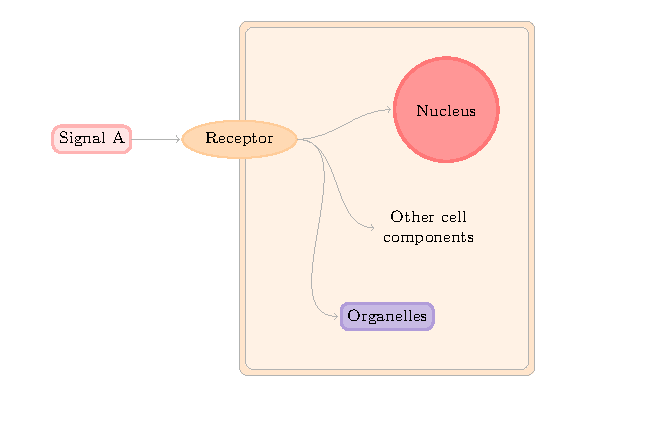
\includegraphics[clip=True, scale=.85]{introduction/signaling_mechanism.pdf}
\end{figure}
\end{frame}


\begin{frame}{Cell Signaling}
A signal propagates in an organism though chemical reactions that are
caused by the change of concentration of chemical species.

\pause
We call the path of a signal a \alert{cell signaling pathway}.
\end{frame}


\begin{frame}{Cell Signaling Pathways}
A cell signaling network can be characterized by a sequence of chemical 
reactions 
\begin{figure}
    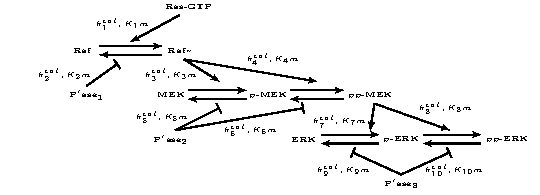
\includegraphics[scale=1.2, trim={.5cm 0 0 0}, clip]{introduction/csp_example.pdf}
\end{figure}
\end{frame}

\begin{frame}{Mathematical Models of Signaling Networks}
We can summarize the state of the cell with measurements based on the 
concentration of some chemical species.
\pause

Using biochemical and enzymatic kinetics, \alert{we can model the 
concentration change of chemical species over time} of a pathway.
\end{frame}


%\begin{frame}{Mathematical Models of Signaling Networks}
%As an example, for the chemical reaction
%\begin{equation*}
%\ce{
    %A -> B
%},
%\end{equation*}

%\pause
%we can write the following equation:
%\begin{equation*}
        %\frac{d[\text{A}]}{dt} = k_1[\text{A}]; 
%\end{equation*}
%where $k_1$ is a reaction rate constant.

%\pause
%Repeating this procedure for all reactions of a pathway allows us to 
%derive a system of ordinary differential equations that can model the 
%signaling pathway.
%\end{frame}


\begin{frame}{Identification of Cell Signaling Pathways}
The problem of identification of cell signaling pathways is the problem
of finding the components of a signaling pathway and how they interact
given a set of experimental measurement.

\pause
As the input, a description of a biological experiment and a set of 
experimental measurements are given. \pause A possible output to the 
problem is composed by:
\begin{itemize}
    \pause
    \item{a model composed by a set of chemical reactions that are 
        relevant for the biological experiment;}
    \pause
    \item{information about the reaction rate constants of the model.}
\end{itemize}
\end{frame}


\begin{frame}{Identification of Cell Signaling Pathways}
One can search for the set of chemical reactions relevant for a 
biological experiment in repositories like the Kyoto Encyclopedia of 
Genes and Genomes (KEGG). \pause However, the pathway maps from KEGG may
be incomplete or have impertinent reactions for the biological 
experiment of interest.
\pause

Hence, it is desirable to construct a method that can systematically 
modify these models and choose the one that better represents the 
experiment.
\end{frame}


\begin{frame}{Identification of Cell Signaling Pathways}
Lulu Wu (2015) presented in her master dissertation a methodology that 
proposes to systematically modify models of signaling network in order
to better represent experiments.
\pause

On her work, the problem of identification of cell signaling pathways is
treated as a feature selection problem.
\end{frame}


%\begin{frame}{Feature Selection Problem}
%The feature selection problem is a combinatorial optimization problem:
%\begin{center}
%Given a set of features $S$ and a cost function $c$, find subset 
        %$X \in \powerset (S)$, with minimum cost $c(X)$.
%\end{center}

%\pause
%\begin{figure}
    %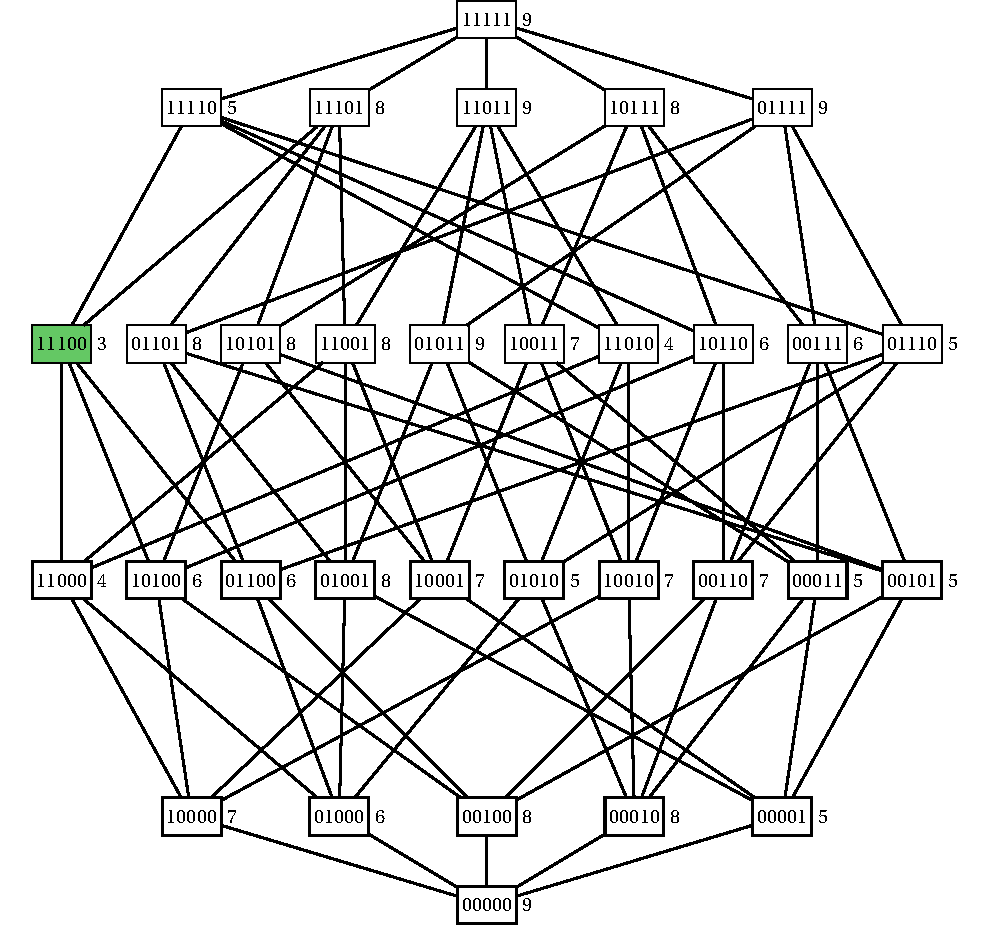
\includegraphics[scale=.24]{introduction/Boolean_lattice.pdf}
    %\caption{An example of feature selection search space with 5 
    %features.}
%\end{figure}
%\end{frame}


\begin{frame}{Feature Selection for Identification of Signaling 
Pathways}
The methodology proposed by Wu defines the set of features as a set of 
chemical reactions that can be added to a starting model.\pause This set 
of chemical reactions is fetched from KEGG and stored in a database of
interactions.
\end{frame}


\begin{frame}{Wu's Search Algorithm for Feature Selection}
The search algorithm used by Wu is the Sequential Forward Selection 
(SFS).
\end{frame}


\begin{frame}{Wu's Cost Function for Feature Selection}
Wu defines the cost function as the minimum distance between 
experimental and simulated data. 
\pause
The minimum distance is found using a Simulated Annealing 
that traverses the parameter space.
\end{frame}


%\begin{frame}{Wu's Cost Function for Feature Selection}
%If we define that:\pause
%\begin{itemize}
    %\item{the experimental measurement is $D$;} \pause
    %\item{the simulated measure is $\phi (M, \theta)$;} \pause
    %\item{all elements visited on the Simulated Annealing process 
        %define $\Theta'$.}
%\end{itemize}
%\pause
%Then, the cost function used on Wu's work is:
%\begin{equation*}
    %c (M) = min_{\{\theta \in \Theta' \subset \Theta\}}  
        %dist (\phi(M, \theta), D) + R (M),
%\end{equation*}
%\pause
%where $R (M)$ is a regularization function.
%\end{frame}


%\begin{frame}{Wu's Cost Function for Feature Selection}
%The $R (M)$ term is implicitly defined by imposing a time limit to the 
%Simulated Annealing procedure used to calculate the cost function. 
%\pause As a result, the penalization of the cost function is random.
%\end{frame}


\begin{frame}{Results of Wu's Methodology}
Lulu Wu tested her methodology by trying to recreate models given a cut
of the original model. \pause However, the methodology worked 
satisfactorily only when the cut was similar to the original model.
\end{frame}


\begin{frame}{Difficulties of Wu's Methodology}
We can point three aspects of Wu's work that could explain its 
limitations.
\begin{itemize}
\pause
\item{the database of interactions used could be more nearly complete;} 
\pause
\item{the search algorithm could also consider removing interactions;}
\pause
\item{the cost function could implement a proper penalization of 
models;}
\end{itemize}
\end{frame}


\begin{frame}{What we Propose on this Project}
We propose to create a methodology that uses a feature selection 
approach for identification of signaling pathways, tackling the 
difficulty of \alert{penalizing complex models}.
\end{frame}

\begin{frame}{What we Propose on this Project}
We intend to use Bayesian approaches of model selection that allow us to
create estimates of $p (M | D)$ or $p (D | M)$.
\end{frame}

\begin{frame}{Objectives of this Project}
\begin{itemize}
\pause
\item{Study state of the art Bayesian algorithms for signaling network
    model selection.}
\pause
\item{Implementation and comparison of cost functions for model
    selection.}
\pause
\item{Formulate systematic modifications to a model as the search space
    of a feature selection model.}
\pause
\item{Observe the surface induced by the cost function over the search
    space.}
\end{itemize}
\end{frame}


%Fundamental Concepts
%- How are the experimental measures taken
    %- A few details about the procedure
%- How can we model cell signaling pathways mathematically
    %- kinetics laws
    %- M.M. simplifcations
%- How can we choose between models
    %- Approximate Bayesian Computation
    %- Annealing-Melting Integration
\section{Fundamental Concepts}
%\begin{frame}{Experimental Measurements of Cell Signaling Pathways}
%Experimental measurements of signaling pathways usually represent the
%ratio of chemical species over time. \pause It is possible to get these
%measurements using a Western blot procedure.
%\begin{figure}
%\end{figure}
%\end{frame}

\begin{frame}{}
\begin{center}
\texttt{Kinetics Modeling of Chemical Reactions}
\end{center}
\end{frame}

\begin{frame}{Mathematical Modeling of Reactions}
In this project we use three possible models of kinetics of an 
interaction:
\begin{itemize}
\pause
\item{first order interaction kinetics;}
\pause
\item{second order interaction kinetics;}
\pause
\item{Michaelis-Menten enzymatic kinetics.}
\end{itemize}
\end{frame}


\begin{frame}{Kinetic Modeling of First Order Iteration}
A first order reaction:
\begin{figure}
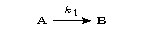
\includegraphics[scale=1.5]{fundamental_concepts/first_order_reaction.pdf}
\end{figure}
\pause
has rate of:
\begin{equation*}
k_1[\text{A}].
\end{equation*}
\end{frame}

\begin{frame}{Kinetic Modeling of Second Order Iteration}
A second order reaction:
\begin{figure}
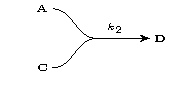
\includegraphics[scale=1.5]{fundamental_concepts/second_order_reaction.pdf}
\end{figure}
\pause
has rate of:
\begin{equation*}
    k_2[\text{A}][\text{C}].
\end{equation*}
\end{frame}


%A simple enzymatic equation can be written as:
\begin{frame}{Kinetic Modeling of Enzymatic Reactions}
An enzymatic reaction:
\begin{figure}
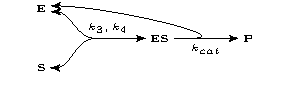
\includegraphics[scale=1.5]{fundamental_concepts/enzymatic_reaction.pdf}
\end{figure}
\pause
Can be divided in two first order reactions plus a second order 
reaction.
\pause
However, with the appropriate assumptions, it is possible to use a 
Michaelis-Menten simplification of this reaction.
\end{frame}


\begin{frame}{Michaelis-Menten Kinetics}
We denote Michaelis-Menten simplification of the last enzymatic reaction
as
\begin{figure}
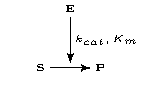
\includegraphics[scale=1.5]{fundamental_concepts/michaelis_menten_reaction.pdf}
\end{figure}
\pause
and it has rate of:
\begin{equation*}
    k_{cat} \frac{[\text{E}][\text{S}]}{K_M + [\text{S}]}.
\end{equation*}
\end{frame}


\begin{frame}{Kinetics of a System of Reactions}
Suppose we want to model the kinetics of A on these reactions:
\begin{figure}
    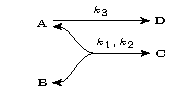
\includegraphics[scale=1.5]{fundamental_concepts/system_reactions.pdf}
\end{figure}
This system can be divided in three reactions:
\begin{itemize}
    \pause
    \item{\ce{A + B -> C}, with rate $k_1[\text{A}][\text{B}]$,}
    \pause
    \item{\ce{C -> A + B}, with rate $k_2[\text{C}]$,}
    \pause
    \item{\ce{A -> D}, with rate $k_3[\text{A}]$.}
\end{itemize}
\end{frame}

\begin{frame}{Kinetics of a System of Reactions}
In \ce{A + B -> C}, with rate 
{\color{red!80!black}$k_1[\text{A}][\text{B}]$}, A is a reactant.
\pause

In \ce{C -> A + B}, with rate 
{\color{green!50!black}$k_2[\text{C}]$}, A is a product.
\pause

In \ce{A -> D}, with rate 
{\color{red!80!black}$k_3[\text{A}]$}, A is a reactant.
\pause

Then, the differential equation that models the concentration change of 
A is:
\pause
\begin{equation*}
    \frac{d[\text{A}]}{dt} = 
        {\color{red!80!black}- k_1[\text{A}][\text{B}]}
        {\color{green!50!black}+ k_2[\text{C}]}
        {\color{red!80!black}- k_3[\text{D}]}.
\end{equation*}
\end{frame}


\begin{frame}{}
\begin{center}
\texttt{Bayesian Methods for Biochemical Model Selection}
\end{center}
\end{frame}

\begin{frame}{State of the Art Methods for Model Selection}
There are two main Bayesian methods available for biochemical model 
selection:
\begin{itemize}
\pause
\item{Approximate Bayesian Computation;}

\pause
\item{Marginal likelihood estimation through Thermodynamic Integration.}
\end{itemize}

\pause
For both methods, we resort to Metropolis-Hastings algorithm to generate
samples of distributions.
\end{frame}


\begin{frame}{Metropolis-Hastings algorithm}
With Metropolis-Hastings, we can generate a sample of a distribution 
$p(\lambda)$ doing the following:
\pause
    \begin{enumerate}
        \pause
        \item{Choose some $\lambda_0$ for which $p (\lambda_0) > 0$, and
            set $t = 1$;}

        \pause
        \item{Sample a candidate point $\lambda^*$ from a jump 
            distribution, $J (\lambda | \lambda_{t-1})$;}

        \pause
        \item{Calculate the ratio 
            $r = \frac{p (\lambda^*) J_t (\lambda^{t - 1} | \lambda^*)}
            {p (\lambda^{t - 1}) J_t (\lambda^* | \lambda^{t - 1})}$;}

        \pause
        \item{Set $\lambda_t = \lambda^*$ with probability $\min (1, r)$
            and $\lambda_t = \lambda_{t-1}$ otherwise;}

        \pause
        \item{Increase $t$ by one and repeat from Step 2 if not reached
            iteration limit.}
    \end{enumerate}
\end{frame}

%Model Selection
%- Approximate Bayesian Computation
    %- What does it do;
    %- ABC-SMC algorithm
%- A method using Thermodynamic Integration
    %- What does it do;
    %- How to derive the thermodynamic integration
    %- How to estimate this value
% Implementations

\section{Model Selection}
\begin{frame}{}
\begin{center}
    \texttt{Ranking with Marginal Likelihood Estimation}
\end{center}
\end{frame}


\begin{frame}{Likelihood of Data Given Model and Parameters}
If we consider that a model $M$ with parameters $\theta$ correctly 
represent the signaling pathway \pause and that there is a Gaussian 
observation error on $D$.
\pause
Then, the likelihood of observing experimental data $D$ is:
\begin{equation*}
     p (D | M, \theta) = \pause 
        p_{\mathcal{N}_{\left(\vec{0}, \Sigma\right)}} 
            (\phi (M,\theta) - D).
\end{equation*}
Where $\phi (M, \theta)$ is the simulated observation.
\end{frame}


\begin{frame}{Marginal Likelihood of Data}
We can marginalize the likelihood to obtain:
\begin{equation*}
    p (D | M) = \int_{\Theta} p (D | M, \theta) p (\theta | M)d\theta
\end{equation*}

\pause
Calculating this integral is hard, therefore we resort to estimating
another integral.
\end{frame}


\begin{frame}{Power-posterior distributions}
We define a power-posterior distribution as:
\begin{equation*}
    p_{\beta} (\theta) = \frac{p (D | \theta, M)^\beta p(\theta | M)}
                    {\int_\Theta p (D | \theta, M)^\beta p(\theta | M) 
                    d\theta},
\end{equation*}
\pause
Note that:

\begin{equation*}
    p_{\beta=0} (\theta) = p (\theta | M),
\end{equation*}

\pause
and that
\begin{equation*}
    p_{\beta=1}(\theta) =\frac{p (D, \theta|M)}
                              {\int_\Theta p (D, \theta | M)d\theta}
                        =\frac{p(\theta | D, M) p(D|M)}{p (D | M)}
                        =p (\theta | D, M).
\end{equation*}
\end{frame}


\begin{frame}{The Thermodynamic Integral}
Using power-posteriors distributions, it is possible to show that
\pause
\begin{equation*}
    \ln p (D | M) = \int_0^1 \expectation_{p_\beta (\theta)} 
        [\ln p(D|\theta, M)]d\beta.
    \label{eq:marginal_likelihood_again}
\end{equation*}
\end{frame}


\begin{frame}{Estimating the Thermodynamic Integral}
It is possible to estimate the Thermodynamic Integral using the 
trapezoidal rule. \pause Setting $0 = \beta_0 < \beta_1 < \ldots 
< \beta_T = 1$, the marginal likelihood is approximately equal to:
\pause
\begin{equation*}
    \footnotesize
    \sum_{t = 0}^{T - 1} (\beta_{t + 1} - \beta_t)
\frac{
    \expectation_{p_{\beta_{t + 1}} (\theta)}[\log p(D | M, \theta)]
+ 
    \expectation_{p_{\beta_{t}} (\theta)}[\log p(D | M, \theta)]}
{2}
\end{equation*}
\end{frame}

\begin{frame}{Estimating the Thermodynamic Integral}
To produce the estimates of 
\begin{equation*}
    \expectation_{p_{\beta_{t}} (\theta)}[\log p(D | M, \theta)]
    \text{ for }
    t \in \{0, \ldots, T\}
\end{equation*}    
we need to produce samples of the 
power-posteriors $p_{\beta_{t}} (\theta)$.
\end{frame}

% Samples are generated running metropolis-hastings for each temperature
% The sampling is divided in three steps. 
%
% On all sampling steps, the proposal distribution is Truncated Normal 
% with only positive numbers
%
% On the first step, the jump distribution used has diagonal covariance
%
% On the second and third step, the jump covariance is estimated with 
% the current sample of the posterior.
%
% On the third step, we use a Populational-MCMC. This method of smapling
% helps mixing chains of different temperature.
\begin{frame}{Sampling from Power-posteriors}
The sampling of the power-posteriors are generated using 
Metropolis-Hastings algorithms in three steps. \pause In all of the 
steps, the proposal distribution used is multivariate log-normal.
\end{frame}


\begin{frame}{Sampling from Power-posteriors}
On the first step, called \alert{naive burn-in} the jump distribution 
has a diagonal covariance matrix. \pause This matrix is updated 
according to the rate of acceptance of parameters.

\pause
\begin{itemize}
\item{if the acceptance rate is high, then increase the variance of the
    jump;}

\pause
\item{if the acceptance rate is low, then decrease the variance of the 
    jump.}
\end{itemize}

\pause
%On the second and third step, the covariance matrix of the jump 
%distribution is estimated with the current sample of the posterior.
\end{frame}

\begin{frame}{Sampling from the Power-posteriors}
On the second sampling step, called \alert{posterior shaped burn-in}, we
use the covariance of the current sample times some constant as the 
covariance of the jump distribution.
\end{frame}

\begin{frame}{Sampling from the Power-posteriors}
On the third step, we perform the \alert{Populational Monte Carlo Markov
Chain} sampling. This algorithm allows us to mix samples from different 
power posteriors.
\end{frame}


\begin{frame}{}
\begin{center}
    \texttt{Ranking with Approximate Bayesian Computation}
\end{center}
\end{frame}


\begin{frame}{Approximate Bayesian Computation}
Approximate Bayesian Computation (ABC) is a method that allows one to
obtain samples of a distribution close to $p (\theta, M | D)$. \pause
A general ABC implementation works as follow:

\begin{enumerate}
    \pause
    \item{Sample a parameter candidate $(\theta^*, M^*)$ from some 
        proposal distribution.}
    \pause
    \item{Generate simulations $\phi (M^*, \theta^*) = D^*$.}
    \pause
    \item{Calculate $d (D^*, D).$ If $d (D^*, D) < \epsilon$ for some 
        previously specified $\epsilon$, then add $(\theta^*, M^*)$ to 
        the sample.}
    \pause
    \item{Repeat until some iteration limit.}
\end{enumerate}
\end{frame}


\begin{frame}{Approximate Bayesian Computation}
The result of the algorithm is a sample of the distribution 
\begin{equation*}
p (\theta, M| d (\phi (M, \theta), D) < \epsilon).
\end{equation*}

\end{frame}

\begin{frame}{ABC Sequential Monte Carlo}
\alert{ABC Sequential Monte Carlo (\texttt{ABC-SMC})} improves a simple
ABC algorithm by using a sequence $\epsilon_0 > \ldots > \epsilon_T$
    acceptance tolerances. 
\pause The sample for a tolerance $\epsilon_i$ is used to generate 
candidates for sample of tolerance $\epsilon_{i + 1}$.

\pause
We can use the accepted parameters of tolerance $\epsilon$ and model $M$
to estimate 
\begin{equation*}
    p (M | d (\phi (M, \theta)) < \epsilon).
\end{equation*}
\end{frame}

\section{Development of SigNetMS}

\begin{frame}{}
\begin{center}
    \texttt{The SigNetMS Software}
\end{center}
\end{frame}

\begin{frame}{A software that estimates the marginal likelihood}
To choose a cost function, we needed to compare the ABC-SMC and Marginal
Likelihood approaches for model selection.
\pause
\begin{itemize}
    \item{\texttt{ABC-SysBio} is a software that implements
        \texttt{ABC-SMC}}
    \item{\texttt{BioBayes} is a software that implements the estimation
        of the marginal likelihood.}
\end{itemize}
\end{frame}

\begin{frame}{A software that estimates the marginal likelihood}
However, the usage of \texttt{BioBayes} in our context was cumbersome.
\pause
Therefore, we decided to implement \alert{SigNetMS}.
\end{frame}

\begin{frame}{The SigNetMS software}
SigNetMS is a Python package and command line software that estimates 
the marginal likelihood of a model given experimental data.
\end{frame}

\begin{frame}{The input expected by SigNetMS}
The input to SigNetMS includes:
\begin{itemize}
    \item{An SBML file model;}
    \item{An XML file with prior distributions of parameters;}
    \item{An XML file with experimental data;}
\end{itemize}
\end{frame}

\begin{frame}{The output produced by SigNetMS}
SigNetMS produces an estimate of the marginal likelihood, as you may
have suspected. \pause Moreover, the software also produces samples of
each power posterior of parameters, which is in turn a sample of the
posterior distribution of parameters.
\pause
\begin{figure}
\centering
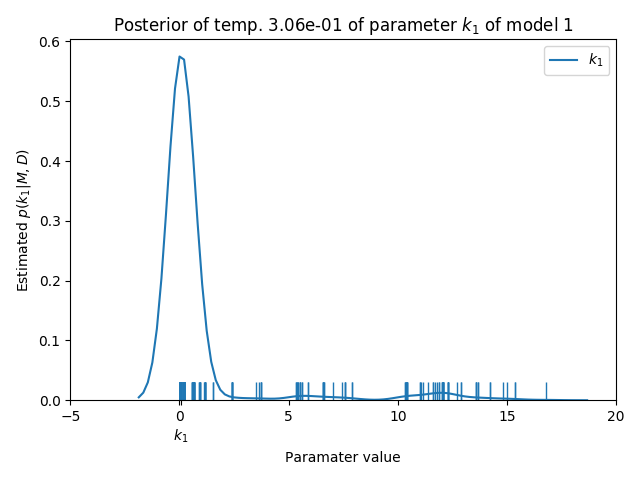
\includegraphics[clip=true,width=.65\linewidth]{experiments/results/girolami/gamma/snm/model1_29_p0_k_1.png}
\end{figure}
\end{frame}

\begin{frame}{}
\begin{center}
    \texttt{Fast integration and parameter sampling}
\end{center}
\end{frame}

% We knew the integration was very expensive
% Talk about the integrator choice
% Talk about symbolic mathematics

\begin{frame}{Problems with efficiency}
To generate a sample to each power posterior, we need to iterate the
Monte Carlo Markov Chain algorithm tens of thousands of times. \pause

For each step we need to evaluate the likelihood function, and 
\alert{numerically integrate the system}. \pause That makes sampling the
most time consuming procedure of SigNetMS.
\end{frame}

\begin{frame}{Our first implementation was not very efficient}
The first implementation of SigNetMS did not cope with larger instances
of model selection. \pause We tackled this problem in two ways:
\begin{itemize}
    \item{change the representation of the system of ordinary
        differential equations;}
    \item{implement parallelization.}
\end{itemize}
\end{frame}

\begin{frame}{Changing the representation of the system of ordinary
differential equations}
In the first implementation of SigNetMS, systems of EDOs were
represented as an array of strings. 

\pause
We used SymPy to provide automatically generated code that allowed us to
create a C function to represent the system of ODEs.
\end{frame}

\begin{frame}{Comparing the representation of the system of ordinary
differential equations}
\begin{table}[]
\centering
\resizebox{\linewidth}{!}{% Resize table to fit within \linewidth horizontally
\begin{tabular}{c c cc}
\hline
\multicolumn{1}{l}{} 
&& \multicolumn{2}{c}{Average time (seconds) to perform a sequence of 
    integrations} \\
\multicolumn{1}{l}{Number of Integrations}               
&& \multicolumn{1}{c}{String Evaluation} 
& \multicolumn{1}{c}{{\tt sympy.autowrap}} \\ \hline 
    10  &&   2.98   & 0.9 \\
    100 && 35.3     & 6.6 \\ 
    200 && 72.1     & 13.1 \\
    400 && 139.1    & 26.9 \\
\hline \hline
\end{tabular}}
\end{table}
\end{frame}

\begin{frame}{Parallelizing the sampling of multiple power posteriors}
The first two phases of the sampling procedure occurs independently
between different power posteriors. \pause

We used the map pattern to parallelize the sampling of different power
posterior distributions. \pause

\begin{figure}[t!]
\begin{center}
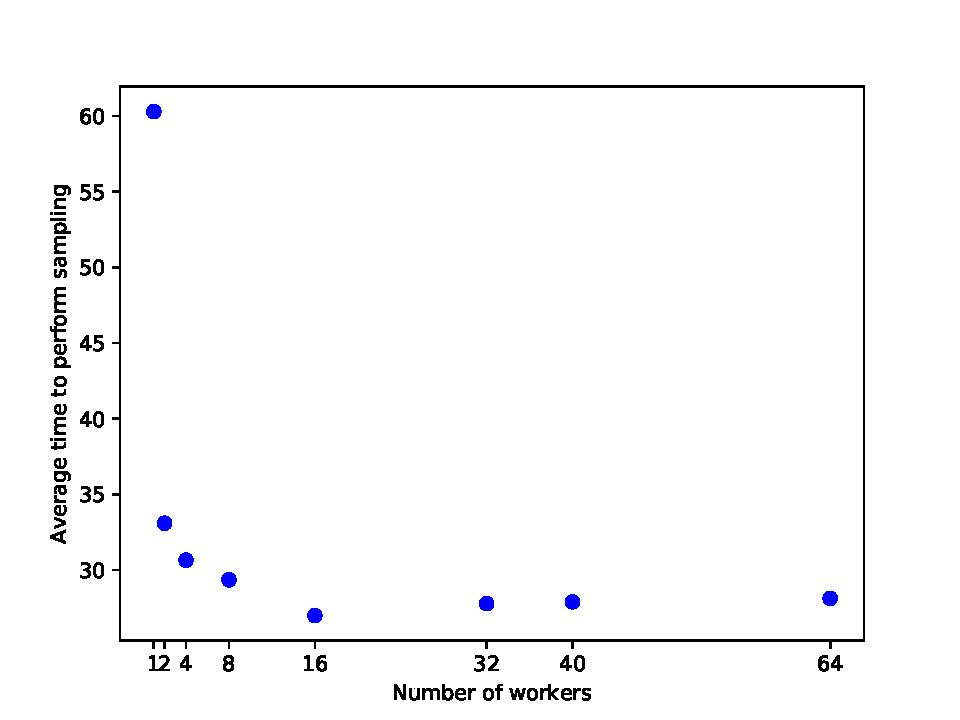
\includegraphics[width=.65\textwidth]{optimizations/workers_experiment.pdf}
\end{center}
\end{figure}
\end{frame}


\section{Experiments and Results}
\begin{frame}{Experiments and Results}
We prepared two experiments in this work: \pause
    \begin{itemize}
        \item{Comparison between ABC-SysBio and SigNetMS}
        \item{Solving model selection as a feature selection instance}
    \end{itemize}
\end{frame}

\begin{frame}{}
\begin{center}
    \texttt{Comparison between ABC-SySBio and SigNetMS}
\end{center}
\end{frame}

\begin{frame}{Choosing a software for model selection}
ABC-SysBio and SigNetMS use different Bayesian approaches for model
selection. \pause The first creates an estimate of $p(M|D)$, \pause and
the second creates an estimate of $p(D|M)$ (the marginal likelihood).
\end{frame}

\begin{frame}{Experiment description}
To compare both software we ran two experiments based on the same 
procedure:
\begin{itemize}
    \pause
    \item{Create 4 candidate models.}
    \pause
    \item{For one of the models, choose a set of parameter values 
        and time steps and simulate data.}
    \pause
    \item{Add Gaussian noise to the simulations. Repeat two more 
        times to generate three observations of the system.}
    \pause
    \item{Neglect chosen parameter values and define prior distributions
        for every parameter.}
    \pause
    \item{Rank the four models.}
\end{itemize}
\pause In this presentation we show results of the first experiment
only.
\end{frame}

\begin{frame}{The instance}
This instance is originally from Vyshemirsky and Girolami (2007), in 
which they present results of Annealing Melting Integration. 
\end{frame}

\begin{frame}{The instance}
\begin{figure}
  \begin{tabular}{c c}
    \subfigure[The ``correct'' model]{
    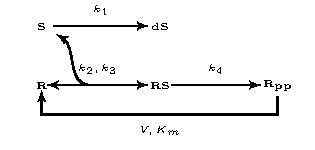
\includegraphics[clip=true,width=.42\linewidth]{experiments/diagrams/bioinformatics_model1.pdf}}
    &
    \subfigure[The simplification model]{
    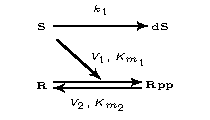
\includegraphics[clip=true,width=.42\linewidth]{experiments/diagrams/bioinformatics_model2.pdf}}
    \\
    \subfigure[The incorrect model] {
    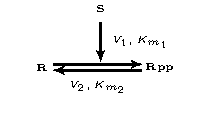
\includegraphics[clip=true,width=.42\linewidth]{experiments/diagrams/bioinformatics_model3.pdf}}
    &
    \subfigure[The generalization model] {
    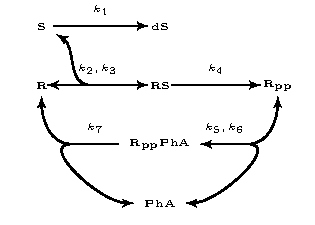
\includegraphics[clip=true,width=.42\linewidth]{experiments/diagrams/bioinformatics_model4.pdf}}
    \end{tabular}
\end{figure}
\end{frame}

\begin{frame}{The instance}
\begin{figure}
\begin{center}
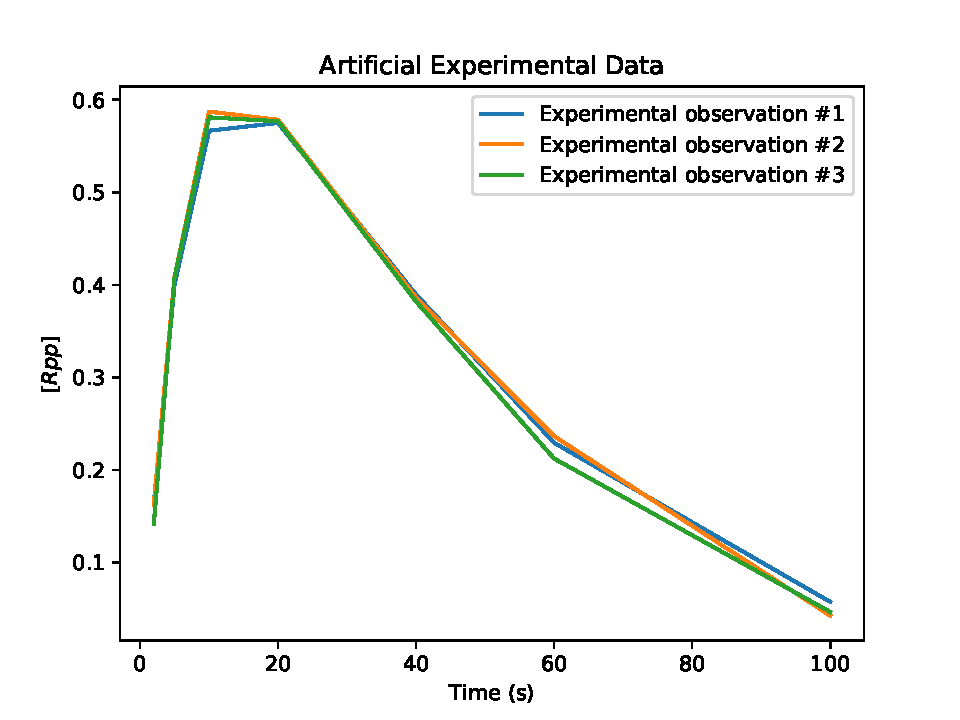
\includegraphics[width=.75\textwidth]{experiments/simulations/girolami_experimental_data.pdf}
\end{center}
\end{figure}

\end{frame}

\begin{frame}{Results on ABC-SysBio}
The ABC-SysBio software returned the following ranking of models:
    \begin{enumerate}
        \pause
    \item{incorrect model}
        \pause
    \item{simplification model}
        \pause
    \item{generalization model}
        \pause
    \item{correct model}
    \end{enumerate}
\end{frame}

\begin{frame}{Results on ABC-SysBio}
\begin{figure}[ht]
    \centering
    \begin{tabular}{c c}
    \subfigure[correct model]{
    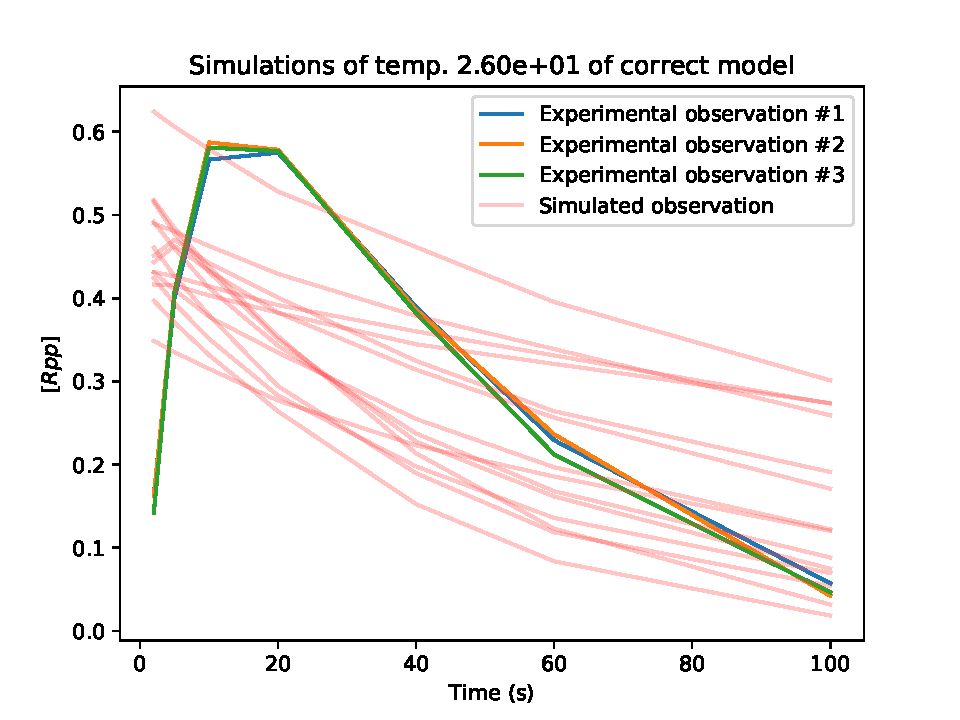
\includegraphics[clip=true,width=.41\linewidth]{experiments/abc_vs_snm/all_model/abc/msimulations_model1_25.pdf}
    \label{fig:girolami_model1_abc}}
    &
    \subfigure[simplified model]{
    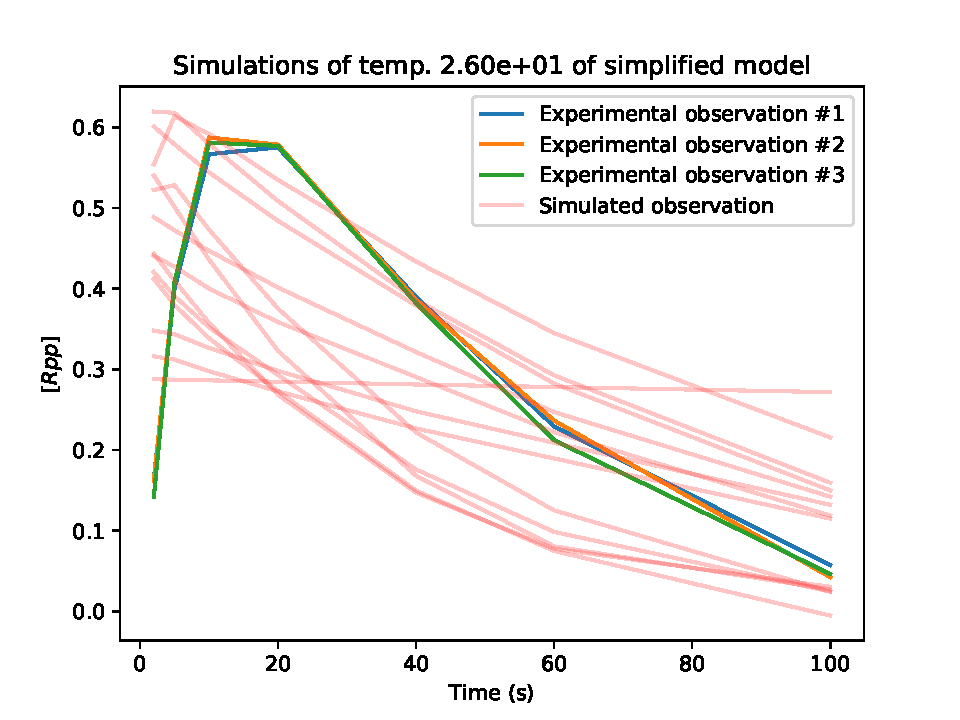
\includegraphics[clip=true,width=.41\linewidth]{experiments/abc_vs_snm/all_model/abc/msimulations_model2_25.pdf}
    \label{fig:girolami_model2_abc}} 
    \\
    \subfigure[incorrect model]{
    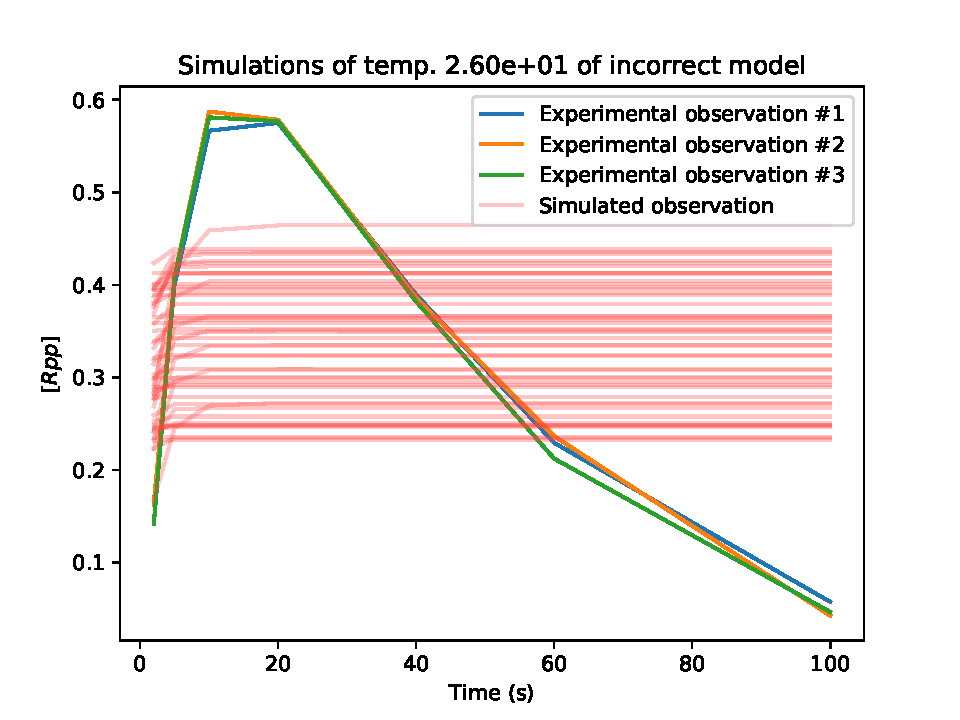
\includegraphics[clip=true,width=.41\linewidth]{experiments/abc_vs_snm/all_model/abc/msimulations_model3_25.pdf}
    \label{fig:girolami_model3_abc}}
&
    \subfigure[generalization model]{
    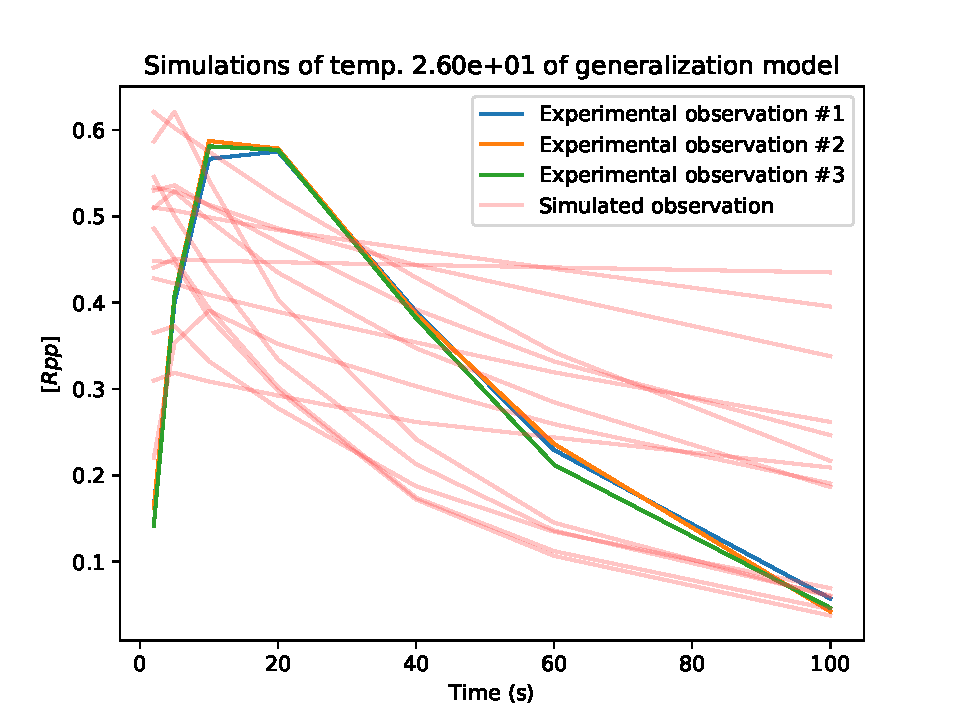
\includegraphics[clip=true,width=.41\linewidth]{experiments/abc_vs_snm/all_model/abc/msimulations_model4_25.pdf}
    \label{fig:girolami_model4_abc}}
    \end{tabular}
\end{figure}
\end{frame}

\begin{frame}{Results on SigNetMS}
The ranking returned by SigNetMS on the first experiment is:
\begin{enumerate}
    \item{correct model}
\pause
    \item{simplification model}
\pause
    \item{generalization model}
\pause
    \item{incorrect model}
\end{enumerate}
\end{frame}

\begin{frame}{Results on SigNetMS}
\begin{figure}[ht]
    \centering
    \begin{tabular}{c c}
    \subfigure[correct model]{
    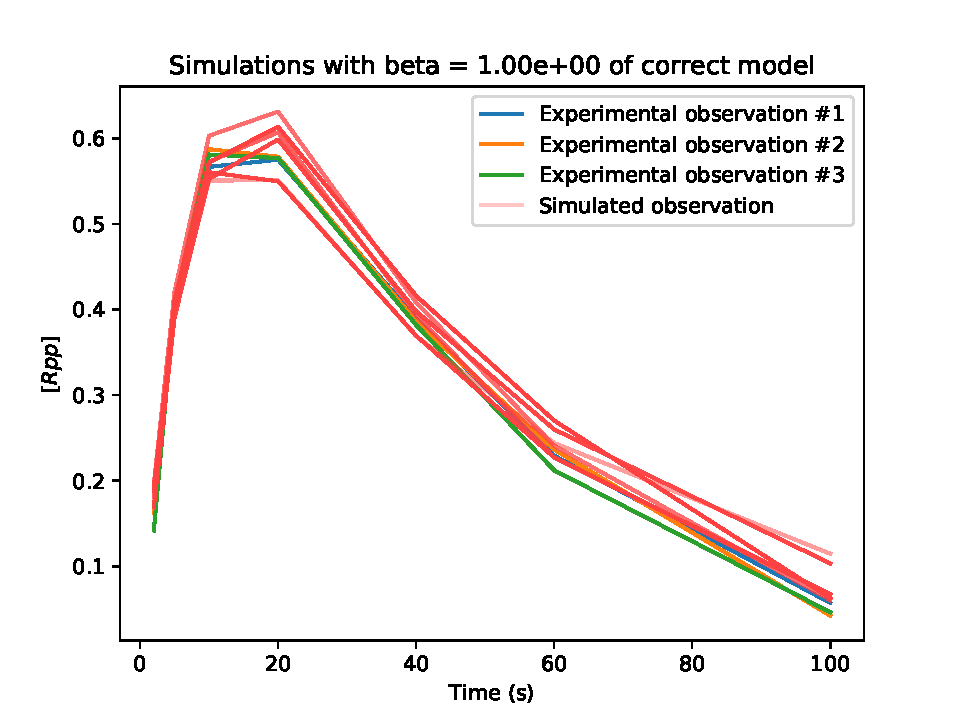
\includegraphics[clip=true,width=.41\linewidth]{experiments/abc_vs_snm/all_model/snm/msimulations_model1_39.pdf}
    \label{fig:girolami_model1_snm}}
    &
    \subfigure[simplified model]{
    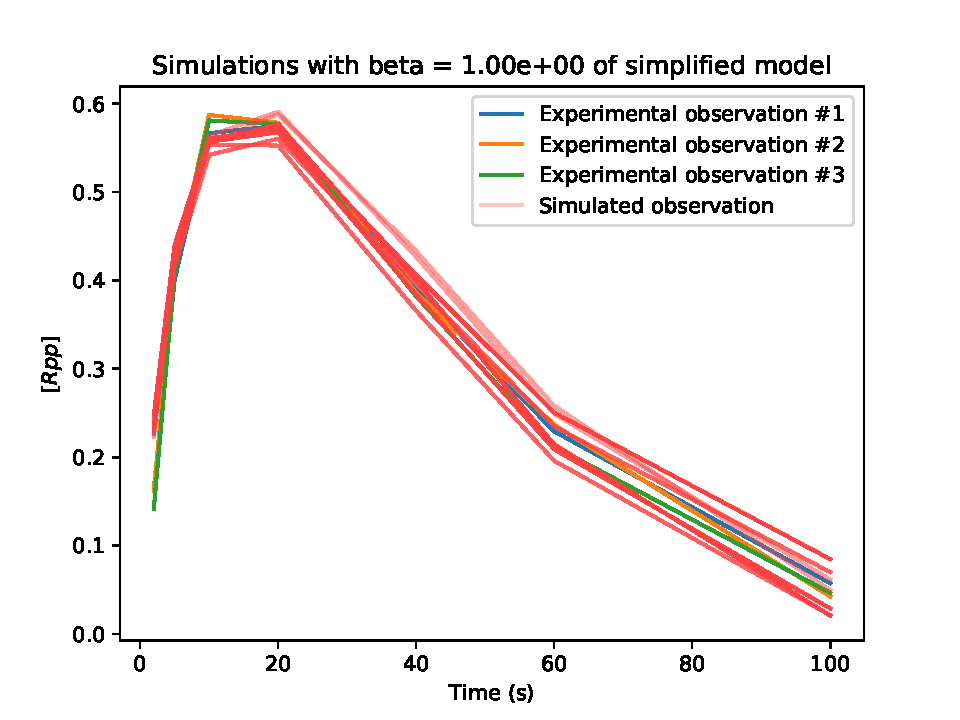
\includegraphics[clip=true,width=.41\linewidth]{experiments/abc_vs_snm/all_model/snm/msimulations_model2_39.pdf}
    \label{fig:girolami_model2_snm}} 
    \\
    \subfigure[incorrect model]{
    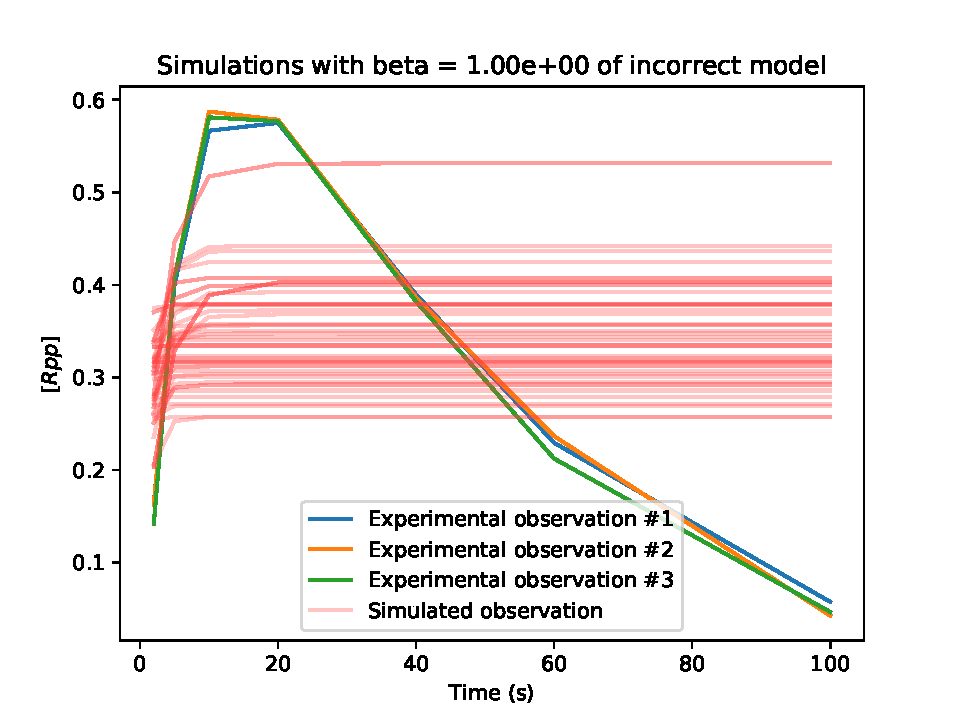
\includegraphics[clip=true,width=.41\linewidth]{experiments/abc_vs_snm/all_model/snm/msimulations_model3_39.pdf}
    \label{fig:girolami_model3_snm}}
&
    \subfigure[generalization model]{
    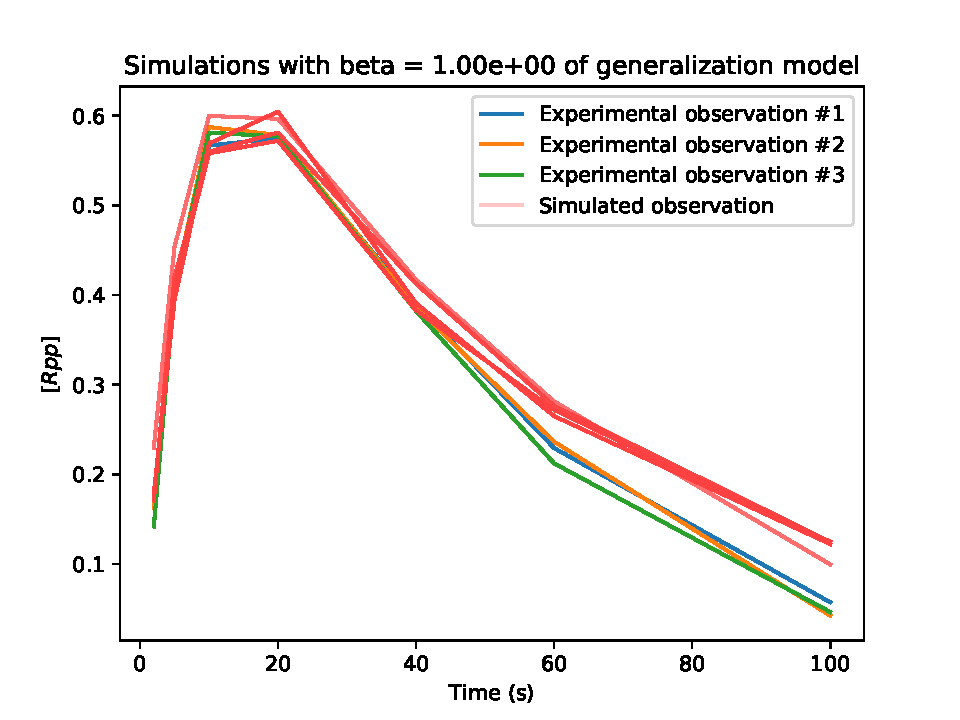
\includegraphics[clip=true,width=.41\linewidth]{experiments/abc_vs_snm/all_model/snm/msimulations_model4_39.pdf}
    \label{fig:girolami_model4_snm}}
    \end{tabular}
\end{figure}
\end{frame}

\begin{frame}
    \href{https://linux.ime.usp.br/~gustavoem/defesa/bioinformatics_correct.gif}
    {Simulations generated by the correct model}
\end{frame}


\begin{frame}{}
\begin{center}
    \texttt{Model selection as a feature selection problem}
\end{center}
\end{frame}

\begin{frame}{Model selection as a feature selection problem}
After defining that SigNetMS is our software choice for a cost function,
we are able to experiment the approach of solving a model selection
instance as a feature selection problem.
\end{frame}

\begin{frame}{The model selection instance}
We proposed a Ras switch pathway to experiment on. \pause
% show the diagram of the correct model

\begin{figure}
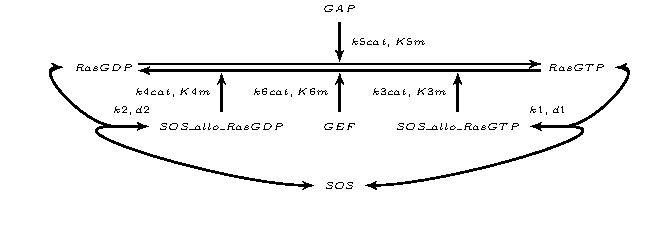
\includegraphics[width=1\textwidth]{experiments/ras_switch/correct.pdf}
\end{figure}
\end{frame}


\begin{frame}{The model selection instance}
% experimental data plot
The concentration of activated Ras was measured at the time steps of 30,
60, 90, 120, 150, 180, 210, and 240 seconds. \pause
\begin{figure}
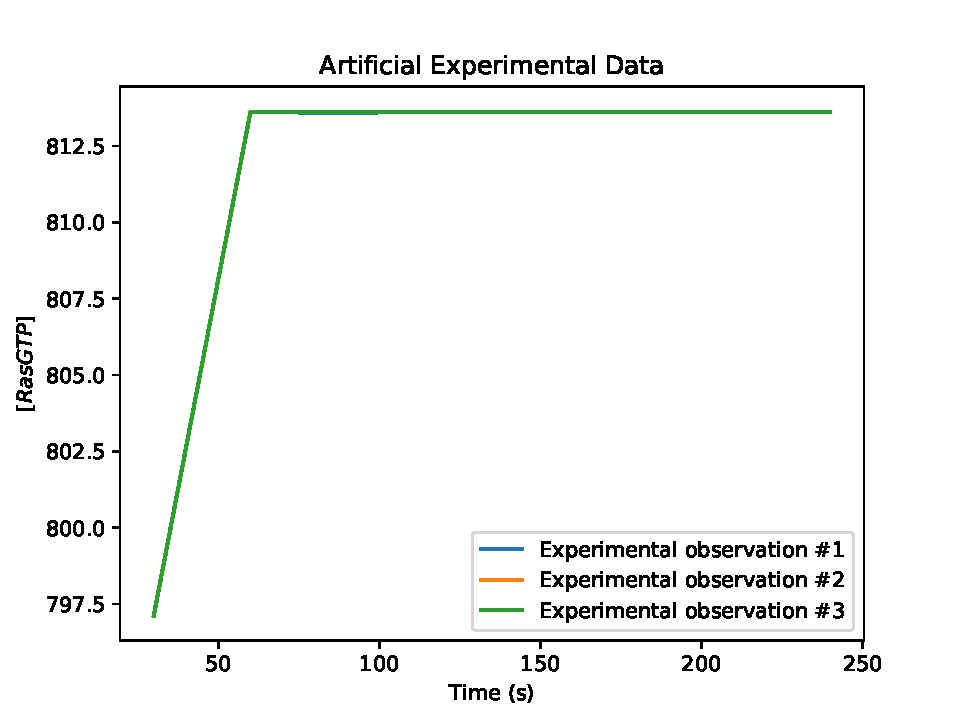
\includegraphics[width=.80\textwidth]{experiments/ras_switch/experiment_plot.pdf}
\end{figure}
\end{frame}


\begin{frame}{Model selection as a feature selection problem}
The feature selection problem consists in finding the best subset of
a set of features, $S$, given a cost function $c$. \pause

If we define the set of feature as a set of reactions, we can create a
feature selection instance that represents a model selection
instance.
\end{frame}


\begin{frame}{Model selection as a feature selection problem}
% figure with the boolean lattice

\begin{figure}[h!]
\begin{center}
    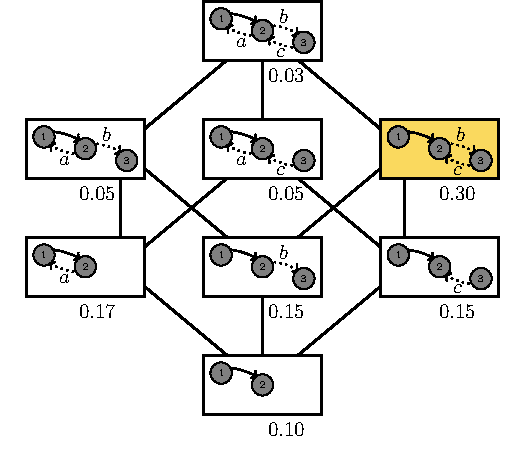
\includegraphics[width=.8\textwidth]{experiments/Boolean_lattice_model_selection.pdf}
\end{center}
\end{figure}
\end{frame}

\begin{frame}{The set of features of our experiment}
In the instance we prepared, the base model has zero reactions, \pause 
and the set of features $S$ is composed by 10 reactions, \pause 8 
of them present on the correct model.
\end{frame}


\begin{frame}{The set of features of our experiment}
% show 4 of the reactions
\begin{figure}[H]
    \centering
    \begin{tabular}{cc}
    \subfigure{
        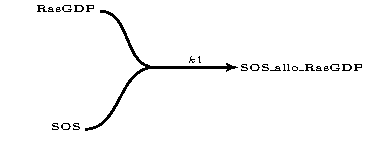
\includegraphics[clip=true,width=.455\linewidth]{experiments/ras_switch/reactions/sos_allo_rasgdp_complexation.pdf}
    }
    &
    \subfigure{
        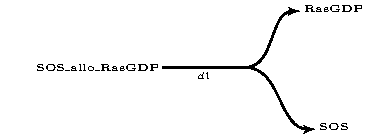
\includegraphics[clip=true,width=.455\linewidth]{experiments/ras_switch/reactions/sos_allo_rasgdp_decomplexation.pdf}
    }
    \\
    \subfigure{
    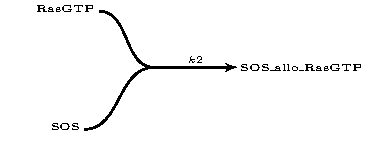
\includegraphics[clip=true,width=.455\linewidth]{experiments/ras_switch/reactions/sos_allo_rasgtp_complexation.pdf}
    }
    &
    \subfigure{
    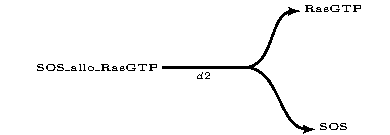
\includegraphics[clip=true,width=.455\linewidth]{experiments/ras_switch/reactions/sos_allo_rasgtp_decomplexation.pdf}
    }
    \end{tabular}
    \label{fig:ras_switch:features}
\end{figure}
\end{frame}


\begin{frame}{The set of features of our experiment}
% show 4 more of the reactions
\begin{figure}[H]
    \centering
    \begin{tabular}{cc}
    \subfigure{
    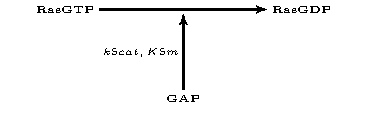
\includegraphics[clip=true,width=.455\linewidth]{experiments/ras_switch/reactions/ras_inactivation_by_gap.pdf}
    }
    &
    \subfigure{
    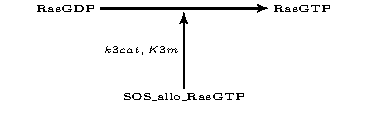
\includegraphics[clip=true,width=.455\linewidth]{experiments/ras_switch/reactions/ras_activation_by_sos_allo_RasGTP.pdf}
    }
    \\
    \subfigure{
    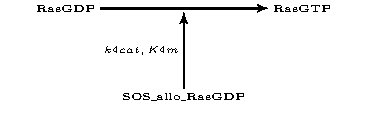
\includegraphics[clip=true,width=.455\linewidth]{experiments/ras_switch/reactions/ras_activation_by_sos_allo_RasGDP.pdf}
    }
    &
    \subfigure{
    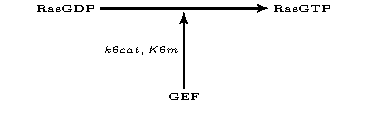
\includegraphics[clip=true,width=.455\linewidth]{experiments/ras_switch/reactions/ras_activation_by_GEF.pdf}
    }
    \\
    \subfigure{
    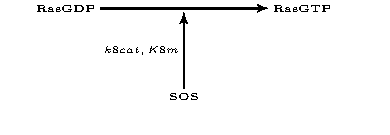
\includegraphics[clip=true,width=.455\linewidth]{experiments/ras_switch/reactions/ras_activation_by_SOS.pdf}
    }
    &
    \subfigure{
    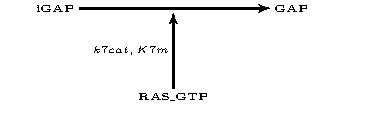
\includegraphics[clip=true,width=.455\linewidth]{experiments/ras_switch/reactions/gap_activation_by_RasGTP.pdf}
    }
    \end{tabular}
\end{figure}
\end{frame}


\begin{frame}{Finding a solution}
% talk about how we used SFS to find a solution
The search space $\powerset(S)$, has $2^{10}$. Therefore, a heuristic 
is necessary to traverse the space. \pause We used the Sequential 
Forward Selection (SFS) algorithm.
\end{frame}


\begin{frame}{Finding a solution}
In the SFS procedure, we start from the bottom of the search space.
\pause And for every iteration, we select the best adjacent model that
has one more reaction.
\end{frame}


\begin{frame}{Results of the search}
% show the trace
% talk about results
\begin{table}
\centering
\begin{tabular}{c|cll}
\hline
Characteristic Vector && \multicolumn{1}{l}{Score} &
\multicolumn{1}{l}{Cost function time (seconds)} \\
\hline
    0000000000 && 330721.05	& 851.3	    \\
    0010000000 && 245681.93	& 1083.4	\\
    0010010000 && 211.62	& 4257.4	\\
    0011010000 && -1.32	    & 5007.71	\\
    0011011000 && -4.27	    & 4458.7	\\  
    \alert{0111011000} && \alert{-7.90}	    & \alert{5035.7}	\\  
\hline
\hline
\end{tabular}
\end{table}
\end{frame}

\begin{frame}{Results of the search}
The found model is contained in the correct model: \pause
\begin{figure}
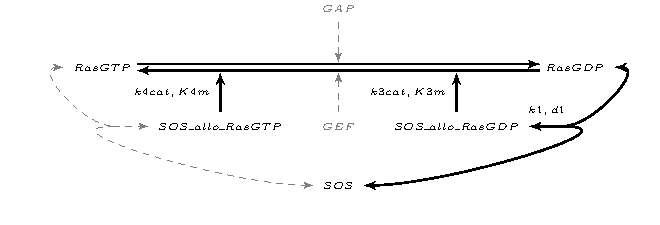
\includegraphics[width=1\textwidth]{experiments/ras_switch/solution.pdf}
\end{figure}
\end{frame}

\begin{frame}{Results of the search}
\href{https://linux.ime.usp.br/~gustavoem/defesa/ras_solution_simulations.gif}
{Simulations generated by the found model}
\end{frame}

\begin{frame}{Results of the search}
\href{https://linux.ime.usp.br/~gustavoem/defesa/ras_correct_model.gif}
{Simulations generated by the correct model}
\end{frame}


\begin{frame}{Results of the search}
In this experiment, we experienced a known feature of marginal
likelihood approaches: \pause \alert{intermediate complexity models are
preferred}.

\begin{figure}
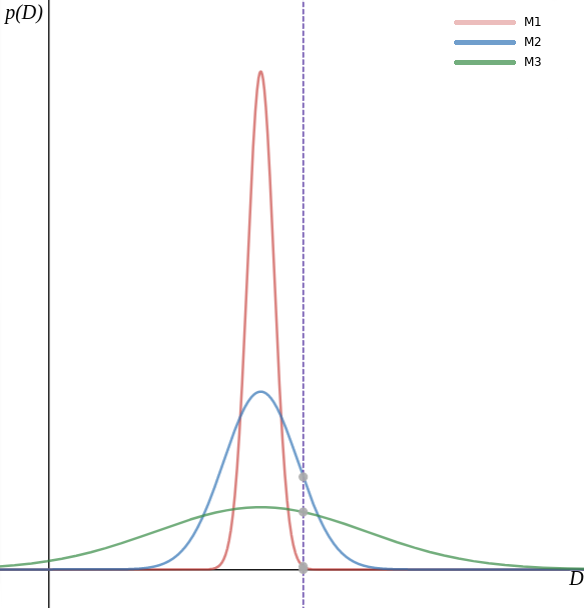
\includegraphics[width=.5\textwidth]{intermediate_complexity_2.png}
\end{figure}
\end{frame}

\section{Conclusions}

\begin{frame}{Contributions of this work}
The main contributions of this work are:
\begin{itemize}
    \pause
    \item{the implementation of the SigNetMS software;}
    \pause
    \item{the comparison between SigNetMS and ABC-SysBio;}
    \pause
    \item{the experimentation of feature selection on model selection
        using a marginal likelihood approach to define the cost
        function.}
\end{itemize}
\end{frame}

\begin{frame}{Suggestions for future work}
We also suggest a few topics for future related work:
\begin{itemize}
    \item{efficiency improvements on SigNetMS;}
        \pause
    \item{treatment of numerical instabilities on numerical integrations
        of SigNetMS;}
        \pause
    \item{solving the model selection problem as a U-Curve problem;}
        \pause
    \item{experimentation on heterogeneous conditions of experimental
        measurements;}
        \pause
    \item{application of the methodology on real instances.}
\end{itemize}
\end{frame}

\begin{frame}{}
\begin{center}
    \texttt{Thank you!}
\end{center}
\end{frame}

\end{document}
